% Options for packages loaded elsewhere
\PassOptionsToPackage{unicode}{hyperref}
\PassOptionsToPackage{hyphens}{url}
\PassOptionsToPackage{dvipsnames,svgnames*,x11names*}{xcolor}
%
\documentclass[
  12pt,
]{article}
\usepackage{lmodern}
\usepackage{setspace}
\usepackage{amssymb,amsmath}
\usepackage{ifxetex,ifluatex}
\ifnum 0\ifxetex 1\fi\ifluatex 1\fi=0 % if pdftex
  \usepackage[T1]{fontenc}
  \usepackage[utf8]{inputenc}
  \usepackage{textcomp} % provide euro and other symbols
\else % if luatex or xetex
  \usepackage{unicode-math}
  \defaultfontfeatures{Scale=MatchLowercase}
  \defaultfontfeatures[\rmfamily]{Ligatures=TeX,Scale=1}
  \setmainfont[]{Times New Roman}
  \setsansfont[]{Times New Roman}
\fi
% Use upquote if available, for straight quotes in verbatim environments
\IfFileExists{upquote.sty}{\usepackage{upquote}}{}
\IfFileExists{microtype.sty}{% use microtype if available
  \usepackage[]{microtype}
  \UseMicrotypeSet[protrusion]{basicmath} % disable protrusion for tt fonts
}{}
\makeatletter
\@ifundefined{KOMAClassName}{% if non-KOMA class
  \IfFileExists{parskip.sty}{%
    \usepackage{parskip}
  }{% else
    \setlength{\parindent}{0pt}
    \setlength{\parskip}{6pt plus 2pt minus 1pt}}
}{% if KOMA class
  \KOMAoptions{parskip=half}}
\makeatother
\usepackage{xcolor}
\IfFileExists{xurl.sty}{\usepackage{xurl}}{} % add URL line breaks if available
\IfFileExists{bookmark.sty}{\usepackage{bookmark}}{\usepackage{hyperref}}
\hypersetup{
  colorlinks=true,
  linkcolor=Maroon,
  filecolor=Maroon,
  citecolor=Blue,
  urlcolor=Blue,
  pdfcreator={LaTeX via pandoc}}
\urlstyle{same} % disable monospaced font for URLs
\usepackage[margin=1in]{geometry}
\usepackage{longtable,booktabs}
% Correct order of tables after \paragraph or \subparagraph
\usepackage{etoolbox}
\makeatletter
\patchcmd\longtable{\par}{\if@noskipsec\mbox{}\fi\par}{}{}
\makeatother
% Allow footnotes in longtable head/foot
\IfFileExists{footnotehyper.sty}{\usepackage{footnotehyper}}{\usepackage{footnote}}
\makesavenoteenv{longtable}
\usepackage{graphicx,grffile}
\makeatletter
\def\maxwidth{\ifdim\Gin@nat@width>\linewidth\linewidth\else\Gin@nat@width\fi}
\def\maxheight{\ifdim\Gin@nat@height>\textheight\textheight\else\Gin@nat@height\fi}
\makeatother
% Scale images if necessary, so that they will not overflow the page
% margins by default, and it is still possible to overwrite the defaults
% using explicit options in \includegraphics[width, height, ...]{}
\setkeys{Gin}{width=\maxwidth,height=\maxheight,keepaspectratio}
% Set default figure placement to htbp
\makeatletter
\def\fps@figure{htbp}
\makeatother
\setlength{\emergencystretch}{3em} % prevent overfull lines
\providecommand{\tightlist}{%
  \setlength{\itemsep}{0pt}\setlength{\parskip}{0pt}}
\setcounter{secnumdepth}{5}
\usepackage{mathtools}

\title{\vspace{1cm}Does Spending Time with Your Child Decreases Your Income?\vspace{0.5cm}\\}
\usepackage{etoolbox}
\makeatletter
\providecommand{\subtitle}[1]{% add subtitle to \maketitle
  \apptocmd{\@title}{\par {\large #1 \par}}{}{}
}
\makeatother
\subtitle{An Investigation on the Causal Effect of Parental Leave on Income in Germany \vspace{0.5cm}}
\author{Sophie Hensgen\\
University of Mannheim\\
Matricle number: 1560750\\
Course: Applied Causal Analysis\\
Lecturer: Paul C. Bauer}
\date{2020-07-15\\}

\begin{document}
\maketitle

\setstretch{1.2}
\hypertarget{introduction}{%
\section{Introduction}\label{introduction}}

In the past 5 years (2015 - 2019) the number of persons which received parental allowance in Germany increased about almost 20 \% from 1,561,597 to 1,865,129. The proportion of men who have benefited from it increased by 3.5\% and now accounts for almost a quarter of those receiving parental benefits. Although there is a continuing trend for more men to take parental leave (PL), there is still a high gender wage gap. Women stay longer in parental leave, in fact on average four times as long as men (Statistisches Bundesamt \protect\hyperlink{ref-statistisches_bundesamt_zeitreihe_2020}{2020}).

Many researchers have addressed this issue to find out whether parental leave could possibly be responsible for the gender wage gap.

The answer? There is no clear answer.
There is evidence that there is an effect of parental leave on income. That said, scholars are indecisive on why this is the case. Some argue, that the time spend in parental leave could lead to decreasing someones knowledge and skill level (Evertsson \protect\hyperlink{ref-evertsson_parental_2016}{2016}). Especially compared to someone which had the same level to begin with. Thus, if they try to re-enter the workforce, they would have to start at a lower position or would be at a disadvantage in terms of promotions due to the missed practice (Gabriele Mari and Cutuli \protect\hyperlink{ref-gabriele_mari_parental_2019}{2019}; Hofferth and Curtin \protect\hyperlink{ref-hofferth_parental_2006}{2006}). This theory is also known as the human capital theory. On the other hand, scholars present another explanation, the signal theory(Albrecht et al. \protect\hyperlink{ref-albrecht_career_1999}{1999}; Evertsson \protect\hyperlink{ref-evertsson_parental_2016}{2016}).
Not only should it explain the difference between persons who been on parental leave and the ones that weren't, but also the differences between genders. As the human capital theory should have the same consequences despite the gender (Evertsson \protect\hyperlink{ref-evertsson_parental_2016}{2016}), the signalling theory tries to explain why there is difference. In principle, the use of parental leave could be seen as less committed to the company. Thus, when it comes to promotions, employers might prefer someone who was not on parental leave to someone who was on parental leave. So some scholar claim, that this signal might be harder on men (Albrecht et al. \protect\hyperlink{ref-albrecht_career_1999}{1999}; Evertsson \protect\hyperlink{ref-evertsson_parental_2016}{2016}; Stafford and Sundström \protect\hyperlink{ref-stafford_time_1996}{1996}), but at the same time other argue that it is more harmful to women (Ridgeway and Correll \protect\hyperlink{ref-ridgeway_unpacking_2004}{2004}). I will go into this in more detail later.

To conclude, scholars are indecisive on what exactly causes the differences. Furthermore, it is not clear whether these factors have long-term effects or not. A number of studies only researches the time frame directly or couple of years after the parental leave and also focus on the employment rate or at how fast someone will find a job again (Pronzato \protect\hyperlink{ref-pronzato_return_2009}{2009}). Which is an important factor to look at, however I am more interested in the differences in income. Despite that there are only few who looked at a rather large period of time. That said, the majority of such research is done primarily in countries other than Germany (Evertsson \protect\hyperlink{ref-evertsson_parental_2016}{2016}). And as the reforms regarding parental leave are different in every country, there could be severe differences in the results (Pronzato \protect\hyperlink{ref-pronzato_return_2009}{2009}).

All in all, I wondered whether the effect of human capital and signal theory might diminish over time. After many years, it might not matter if you missed a year, other aspects might become more important. Alternatively, it could be that one has gained such disadvantages from the parental leave that these could have far-reaching consequences. If the former is true, this could lead to more men taking parental leave because they are less concerned about their career. And this in turn could lead to a decrease in the gender wage gap.
So my question is, is there a long term effect of taking parental leave on income and does the length of the leave has a additional influence?

In the following I will discuss how the parental leave reform in Germany has changed over the years. In addition, what to consider before deciding on whether to take parental leave, as this could lead to self-selection. I will also explain in more detail how human capital and signal theory can be applied to this question. Which I will later investigate in a natural experiment. For this, I will use the difference in differences model with the SOEP Panel Dataset.

\hypertarget{literature-review}{%
\section{Literature Review}\label{literature-review}}

\hypertarget{history-of-parental-leave}{%
\subsubsection*{\texorpdfstring{\emph{History of Parental Leave}}{History of Parental Leave}}\label{history-of-parental-leave}}
\addcontentsline{toc}{subsubsection}{\emph{History of Parental Leave}}

In order to fully understand the impact maternity, paternity and parental leave might have on an individual in Germany, it is necessary to look into the reform itself and how it changed over the years to become more inclusive.

Maternity leave itself did not changed as much, women were guaranteed 14 weeks of leave (6 weeks pre birth and 8 post birth) with full payment of their salary (Gabriele Mari and Cutuli \protect\hyperlink{ref-gabriele_mari_parental_2019}{2019}). In the 1980s, mothers were offered 6 months of paid and job guaranteed leave. This reform has been amended several times. Especially in the 1990s they began to change the status quo substantially. Not only changed the period of time during which a safe return to work was guaranteed to 36 months in 1992. But also they adjusted the financial support in the same year so that it could be paid for up to 18 months. This financial support consisted of a mixture of flat-rate and means-tested payments (Gabriele Mari and Cutuli \protect\hyperlink{ref-gabriele_mari_parental_2019}{2019}). Another rather big change was the possibility that men could also go into parental leave (Ajdacic-Gross \protect\hyperlink{ref-ajdacic-gross_elterngeld_2020}{2020}). Being in parental leave simultaneously was introduced in 2001.

The next substantial reform change took place in 2007. Paid leave was at least 12 months or 14 months if both parents took at least two months parental leave. These additional 2 months should act like an incentive for fathers to take part in parental leave (Gabriele Mari and Cutuli \protect\hyperlink{ref-gabriele_mari_parental_2019}{2019}; Lapuerta, Baizán, and González \protect\hyperlink{ref-lapuerta_individual_2011}{2011}; Marshall \protect\hyperlink{ref-marshall_fathers_2008}{2008}). Also the financial support system changed. If someone was employed to the time of the birth they would get paid 67 \% of their pre-birth net salary. But if they were not employed they would get 300 Euro per month as financial support (Hofferth and Curtin \protect\hyperlink{ref-hofferth_parental_2006}{2006}).

These reform changes have a strong influence on whether fathers take parental leave or not. Before 2007, only 3\% of fathers took parental leave. After 2007, the figure had already risen to 15\%, increasing over the years to 34\% (2014) (Tamm \protect\hyperlink{ref-tamm_fathers_2018}{2018}).
Gabriele Mari and Cutuli (\protect\hyperlink{ref-gabriele_mari_parental_2019}{2019}) examined the impact the 2007 reform had on the income of parents and they found out that indeed, more fathers engaged in parental leave and also that it was easier to return to the job market for women.

\hypertarget{theory-hypotheses}{%
\section{Theory \& Hypotheses}\label{theory-hypotheses}}

\hypertarget{impact-of-parental-leave}{%
\subsubsection*{\texorpdfstring{\emph{Impact of Parental Leave}}{Impact of Parental Leave}}\label{impact-of-parental-leave}}
\addcontentsline{toc}{subsubsection}{\emph{Impact of Parental Leave}}

According to multiple scholars, there is a significant influence of parental leave on income in varying degrees.
However, it should be noted that there are two aspects to be considered. First, there are factors which influence the decision to go into parental leave, which can lead to the overrepresentation of women staying home for their newborn. And secondly, parental leave seems to have a different impact on the sexes (Evertsson \protect\hyperlink{ref-evertsson_parental_2016}{2016}). In the following section, I will first focus on what is involved in the decision-making process about who goes on parental leave and for how long. And then, I will explore the different theories explaining the impact of parental leave and especially the discrepancy between genders.

Taking time to nurture your new born child is an important aspect in the relationship between parents and their child. For a lot of people it is without question that they will take parental leave, even for a longer period of time.
However, the decision which partner takes it must be made with caution. In general, parents usually act rationally in this respect, they weigh their costs and benefits against each other. As the economic theory says (Lapuerta et al. \protect\hyperlink{ref-lapuerta_individual_2011}{2011}). Thus they achieve the best possible result in terms of finances, re-entry into the world of work, etc..
For example, parents look into the labor market and their own company to find out, if the situation is stable and and which partner is more suitable for leaving work for a period of time (Albrecht et al. \protect\hyperlink{ref-albrecht_career_1999}{1999}). However, some decisions which are made during this time even if chosen rationally can lead to disadvantages, for one party, often for women. Research shows that especially first time parents tend to engage in a more traditional constellation {[}dribe\_does\_2009{]}.

These decisions are made on the basis of several criteria and are not only determined by stereotypes of a traditional family. I will go into detail about 6 of them, which seem to be especially prominent.

To begin with the perhaps least crucial criteria is the lifestyle preferences of each individual. For some, work is more important, for some it is the family, for others it is a matter of adapting to the situation. Depending on which side one is on, this can influence the willingness to take parental leave and also the extent to which it is taken (Hakim \protect\hyperlink{ref-hakim_lifestyle_2002}{2002}).

Another aspect I mentioned before is the situation of the labor market. Some parents are worried, that if they take parental leave, they could have disadvantages compared to other workers in this field. Additionally, some markets are more stable than other, so if someone has a secure job, they might feel more confident in leaving for a period of time (Lapuerta et al. \protect\hyperlink{ref-lapuerta_individual_2011}{2011}).
However, this might not be the most influential part, as these concerns are closely linked with the reform which is in action. As for Germany, there is a guaranteed reentry at the company you work at.

Which brings us to the next criteria, parental leave reforms. These are very different in every country, some are more flexible (Finland, Germany), some are not (Spain, Italy, Greece) (Gabriele Mari and Cutuli \protect\hyperlink{ref-gabriele_mari_parental_2019}{2019}; Pronzato \protect\hyperlink{ref-pronzato_return_2009}{2009}; Tamm \protect\hyperlink{ref-tamm_fathers_2018}{2018}). More flexible reforms increase the probability that fathers will take parental leave (Gabriele Mari and Cutuli \protect\hyperlink{ref-gabriele_mari_parental_2019}{2019}).
Nevertheless, the rate of fathers taking parental leave is still low, as society still expects women to stay at home at least initially (Katherine Marshall \protect\hyperlink{ref-katherine_marshall_fathers_2008}{2008}).

This does not necessarily have to have anything to do with sexism and stereotypes, although they do have an impact, but there are practical reasons as well. The woman carries the child, gives birth and would probably also breastfeed it in the first couple of months, if she decide to do so. Therefore it makes sense that the mother stays at home with the child at the beginning (Albrecht et al. \protect\hyperlink{ref-albrecht_career_1999}{1999}). However, this does not explain, why women stay even longer even though both parents could technically care for the child after the two month maternity leave.

However, the tendency is away from the traditional path, especially among parents with higher education. Although people with a high level of education would have higher opportunity costs if they took parental leave because it is easier for them to improve their career and therefore more likely to refrain from taking parental leave, and if for a shorter period, they are more likely to abandon heteronormative standards and adopt more egalitarian gender roles. (Geisler and Kreyenfeld \protect\hyperlink{ref-geisler_against_2011}{2011}; Helen Dearing \protect\hyperlink{ref-helen_dearing_does_2015}{2015}; Lapuerta et al. \protect\hyperlink{ref-lapuerta_individual_2011}{2011}; Rostgaard, Christoffersen, and Weise \protect\hyperlink{ref-rostgaard_parental_2020}{2020}).
With that said, there is one important aspect to note. Even though highly educated men are open to the idea of taking parental leave, it is important, that it is conform with the economic theory. Which means that they are more likely to go into parental leave, if their significant other has a higher education or higher income than themselves (Geisler and Kreyenfeld \protect\hyperlink{ref-geisler_against_2011}{2011}; Lapuerta et al. \protect\hyperlink{ref-lapuerta_individual_2011}{2011}; Sundstrom \protect\hyperlink{ref-sundstrom_gender_2002}{2002}; Tamm \protect\hyperlink{ref-tamm_fathers_2018}{2018}).

In general, income seems to be the most important criteria in relation to parental leave. The person with the higher salary is most likely to not go into parental leave. Additionally, income can determine how long a family will go into parental leave. For example, high-income families can afford to take more time off for parental leave because they do not need a full additional income (Geisler and Kreyenfeld \protect\hyperlink{ref-geisler_against_2011}{2011}).

Once the decision has been made who will take parental leave, that person will most likely bear some disadvantages (Evertsson \protect\hyperlink{ref-evertsson_parental_2016}{2016}).
One of these disadvantages are the missed opportunities at work. Companys are fast changing mechanisms. New structures, workflows and task are added constantly. So missing out on these, even for a small period of time, could be harmful for one's career (Evertsson \protect\hyperlink{ref-evertsson_parental_2016}{2016}). These findings are in line with the human capital theory which states that an individual will increase its knowledge and skills through education and working in a specific field. The longer someone has been working and the more supplementary training and task he completed the higher his or hers human capital will be (Becker \protect\hyperlink{ref-becker_human_1993}{1993}; Evertsson \protect\hyperlink{ref-evertsson_parental_2016}{2016}). A high human capital is especially important to receive great job offerings, a high salary or promotions. Thus, a break in working life can act as a career impediment. Moreover, not only does human capital not increase if people stay at home, but it actually decreases due to lack of practice (Evertsson \protect\hyperlink{ref-evertsson_parental_2016}{2016}). This assumption is supported by the study by Hofferth and Curtin (\protect\hyperlink{ref-hofferth_parental_2006}{2006}). In their results, they found evidence that the salary already decreases 2 years after birth when the employer is changed. Although they have only focused on the impact on women, there are studies like Evertsson (\protect\hyperlink{ref-evertsson_parental_2016}{2016}) which show that both women and men suffer a loss of pay after parental leave.

Despite that, the well being of the child is most important for the parents, and they will only return to work, if it is more valuable for the family when him or her spends time working instead of carrying for the child (Desai and Waite \protect\hyperlink{ref-desai_womens_1991}{1991}; Hofferth and Curtin \protect\hyperlink{ref-hofferth_parental_2006}{2006}; Leibowitz, Klerman, and Waite \protect\hyperlink{ref-leibowitz_employment_1992}{1992}).

So far we explored the impact parental leave can have on human capital, however there is another important theory which might explain the impact parental leave has the signalling theory.

According to signal theory, any action we take send out a signal that allows others to build up certain beliefs about us (Mignot and Manzo \protect\hyperlink{ref-mignot_peter_2011}{2011}). This means that parental leave can be a signal of less commitment to the company and its work, according to the researchers (Stafford and Sundström \protect\hyperlink{ref-stafford_time_1996}{1996}). It is not clear which gender is more affected by it. According to Albrecht et al. (\protect\hyperlink{ref-albrecht_career_1999}{1999}) this seems to be more a problem for men than for women. Caused by the expectation that women will take more care of their newborn child than their husbands is still widespread in society. 25\% of all couples do not even consider the possibility that the man could take parental leave (Rostgaard et al. \protect\hyperlink{ref-rostgaard_parental_2020}{2020}). It is so normalized, that the signal a women gives with taking maternity leave is not that severe and should not influence her income as much (Ridgeway and Correll \protect\hyperlink{ref-ridgeway_unpacking_2004}{2004}). However, if a man decides to take parental leave, this is still considered an exception. Especially in the period before 2007, when there were no additional incentives for men. So any time spend in parental leave will signal the employer that the father has even less determination for the company (Albrecht et al. \protect\hyperlink{ref-albrecht_career_1999}{1999}; Evertsson \protect\hyperlink{ref-evertsson_parental_2016}{2016}).

This is supported by the Swedish study by Stafford and Sundström (\protect\hyperlink{ref-stafford_time_1996}{1996}) where it was observed that men will experience an annual loss of 5.2\% of pay, but women will lose only 1.7\% of their income. Also, the salary has a great influence how impactful parental leave can be. The higher the income at the time of birth, the less the use of parental leave affects future income (Stafford and Sundström \protect\hyperlink{ref-stafford_time_1996}{1996}). Those results were examined for a shorter time period.

So taking both theories as well as the prior research into account, I believe, that taking parental leave in general will have a long-term effect in your income. The reason being that due to the short-term effects of missed opportunities and the resulting reduction in pay, missed promotion or a generally lower position than before, the career could be dramatically affected.
Therefore I propose the following hypothesis:

\emph{H1: Parental leave has a long-term negative effect on income}

Taking no parental leave should have no effect on the future income, only having a child in general might effect the income, however, that is not to be expected.

Another important question for parents is how long they decide to stay in parental leave, as it has such an impact financially and career wise.
Most scientists are largely of the same opinion, namely that the longer a parent is absent from work, the stronger are the negative effects (Evertsson \protect\hyperlink{ref-evertsson_parental_2016}{2016}; Helen Dearing \protect\hyperlink{ref-helen_dearing_does_2015}{2015}; Pronzato \protect\hyperlink{ref-pronzato_return_2009}{2009}; Rostgaard et al. \protect\hyperlink{ref-rostgaard_parental_2020}{2020}). Additionally, there seems to be a sweet spot where parental leave has a positive effect on mothers later employment participation, but does not have a positive effect on the income (Plantenga and Remery \protect\hyperlink{ref-plantenga_reconciliation_2005}{2005}; Pronzato \protect\hyperlink{ref-pronzato_return_2009}{2009}). Platenga found that the effect behaved in an inverted U shape. Very short and very long leaves seem to have less of a positive effect than a moderate period of time.
However, it is not clear what what concludes a moderate length, they vary across researches. Some say 6-8 months (Plantenga and Remery \protect\hyperlink{ref-plantenga_reconciliation_2005}{2005}) others go up to 18 months (Misra, Budig, and Boeckmann \protect\hyperlink{ref-misra_work-family_2011}{2011}).

Additionally, Rostgaard et al. (\protect\hyperlink{ref-rostgaard_parental_2020}{2020}) even go so far as to propose that a really short time of parental leave could have no long term effect on income, as long as the parental leave, does not change the basic family dynamic. With that said, human capital theory as well as the signalling theory propose that any length lead to a change. Additionally, Evertsson (\protect\hyperlink{ref-evertsson_parental_2016}{2016}) also found a long term effect on the income on women as they take longer time of than men. Suggesting, that it really does care how long one is staying in parental leave regarding long term effects.

Consequently, I suggest, that a long leave period will have a long term negative effect on income. And subsequently a short leave should have no or positive effects. The reason being, that although the parents want to care for their child, they also want to work. This shows a degree of commitment and flexibility as they adapt quickly to a new situation.

Thus the following hypothesis:

\emph{H2: taking a long parental leave will have negative long-term effects on the income.}

All the aspects considered on who will take parental leave lead to women being forced into the traditional role of a mother.
And even though governments try to counterbalance this effect with longer and higher financial support during the parental leave as well as incentives for men to take it, there is still a large gender gap (Helen Dearing \protect\hyperlink{ref-helen_dearing_does_2015}{2015}; Marshall \protect\hyperlink{ref-marshall_fathers_2008}{2008}; Rostgaard et al. \protect\hyperlink{ref-rostgaard_parental_2020}{2020}).
This gap will ultimately lead to an even higher gender wage gap.
Contrary to the research done on signalling theory that man suffer from more disadvantages because of the parental leave (Albrecht et al. \protect\hyperlink{ref-albrecht_career_1999}{1999}). I would argue, that women do as well. It starts with the fact that employer anticipate women to go into parental leave at least ones, solely because they are women. They will believe that women as soon as they get pregnant will be less committed to the company. And if they really go into parental leave, these beliefs of the employer might reinforce even though the woman did nothing to give this particular signal (Ridgeway and Correll \protect\hyperlink{ref-ridgeway_unpacking_2004}{2004}). And in combination with the decrease in human capital women will have even less of a chance to compete with their male counterparts for certain positions. Especially with regard to long-term effects. The signal effect may be short-lived, but on the one side could the short term effects have long term consequences. And on the other side the loss of human capital will continue to affect the career and especially as men have better chances to start with. I therefore believe that women will be at a greater disadvantage than men when it comes to taking parental leave. Men will be affected by the parental leave, however the effect will be not as strong as for women.
Therefore I propose the following hypothesis:

\emph{H3: Being a mother and taking parental leave will have additional negative effect on their income.}

\hypertarget{methods-data}{%
\section{Methods \& Data}\label{methods-data}}

\hypertarget{ideal-study}{%
\subsection*{\texorpdfstring{\emph{Ideal Study}}{Ideal Study}}\label{ideal-study}}
\addcontentsline{toc}{subsection}{\emph{Ideal Study}}

There are several ways to investigate the long-term effects of parental leave on income. One of them would be conducting a difference in differences model. Where we compare the treatment group, in this case parents which take parental leave with the control group parents which did not take parental leave.

In an ideal scenario there would be complete randomness when assigning one to the treatment or control group. But because getting pregnant and ultimately choosing whether to go into parental leave or not is a heavily self selected process it would need correction. One possible way to do so would be to randomly manipulate peoples' contraception. Thus, couples would not be able to control whether they get pregnant or not, so children would be randomly assigned.

To counter balance the criteria which will be considered during the decision process, we would need to perfectly match both groups on gender, age, educational level, work field, income, working hours, relationship status, year of birth, number if children, number of previous parental leaves and their length and region of living.
In regards to the study design, it would be the best if the variables which are used to match the groups and the outcome variable would be examined prior to the pregnancy (t1), therefore the income should not be affected. However, t1 should not be to far in advance, so it would be best, when they would become pregnant right after the first observation. After 30 years I would look at the income from both the control and treatment group and look at the difference in income, given, that they still able to work. If they went early in pension, the last income before that would be considered. I believe that after 30 years the children are grown up and do not need any further support, thus the parents had the opportunity to work again for a longer period of time. Moreover, the possibility to observe a very long period of time gives a better indication on long-term effects.

\hypertarget{method}{%
\subsection*{\texorpdfstring{\emph{Method}}{Method}}\label{method}}
\addcontentsline{toc}{subsection}{\emph{Method}}

Unfortunately, it is not possible nor ethical correct to conduct the study in the extent I proposed earlier, thus I choose a more simple approach to explore the effects of parental leave.

I will conduct a natural experiment in order to test whether there is a causal effect of parental leave on income or not. Hereby I rely on the parallel trend assumption, as I would argue that people who are going into parental leave would have the same development in their careers if they had chosen not to partake in parental leave.\\
To examine this assumption I will use a difference in differences model, where the treatment is whether someone is taking parental leave (\emph{first hypothesis}), is staying for a long period of time (\emph{second hypothesis}) or taking parental leave as a woman (\emph{third hypothesis}).
The outcome variable, income, is measured at two different points in time, 15 years apart. The reason I choose 15 years over 30 is, that with that I can ensure a higher sample. However this could be something future research will concentrate on. This is to ensure that a long-term effect is examined. The control variables are also measured at the first time point (t1) and the treatment variable is measured the following year.
To estimate the causal inference a linear regression is used based on the following equation.

\[y_t - y_{t-1} = \beta_0 + \beta_{treatment} D + \beta_{control} X + \epsilon \]

\hypertarget{data}{%
\subsection*{\texorpdfstring{\emph{Data}}{Data}}\label{data}}
\addcontentsline{toc}{subsection}{\emph{Data}}

In regards to the data, I will use the German Socio-Economic Panel (SOEP) data set. This is a panel data set, which was conducted every year between 1984 to 2018 by the DIW Berlin\footnote{Deutsches Institut für Wirtschaftsforschung}(Liebig et al. \protect\hyperlink{ref-liebig_socio-economic_2019}{2019}). The sample was collected via a random route procedure in German households and combines annually 30,000 individuals in 15,000 households.

I will only use a subset of this data set which includes participants that had a child between 1995 to 2000. The reason why I limit myself to these years is that on the one side the parental leave variable was firstly introduced in 1996 referencing to 1995.
On the other hand, I would not have been able to study the long-term effects of parental leave. The reason for this is that people who took part in the survey at t1 were often no longer represented at t2.
This is especially true for the years after 2000. Furthermore, some variables were changed or omitted from the survey after 2000.
I also excluded participants which were younger than 21 or older than 50 years. This ensures that they had the opportunity to work, both before the pregnancy and 15 years later. I also deleted parents (10 particpants) which had more then one child born in the years between 1995 and 2000 in order to prevent any bias caused by this.

\hypertarget{dependent-variable}{%
\subsubsection*{\texorpdfstring{\emph{Dependent Variable}}{Dependent Variable}}\label{dependent-variable}}
\addcontentsline{toc}{subsubsection}{\emph{Dependent Variable}}

The dependent variable for this study is income and to examine it I use the generated annual income variable by the SOEP team. The variable consists off of all annual labor earnings including ``wages and salary from all employment including training, primary and secondary jobs, and self-employment, plus income from bonuses, overtime, and profit-sharing'' on a continuous level (Grabka \protect\hyperlink{ref-grabka_soep_2017}{2017}:9). I include all labor earnings as I believe that the impact of parental leave is not limited to the salary. However, I deleted extreme outliers, as they could bias the whole outcome especially with such a small sample. Now the range for the income at t1 is between 0 and 75,000, the mean hereby is by ca. 21,000 Euros (shown in Table \ref{tab1}). The income at t2 is higher overall, with a range between 0 and ca. 130,000 euros. This is due to the fact, that income will naturally increase with age (CITE).

\hypertarget{independent-variables}{%
\subsubsection*{\texorpdfstring{\emph{Independent Variables}}{Independent Variables}}\label{independent-variables}}
\addcontentsline{toc}{subsubsection}{\emph{Independent Variables}}

The variable which displays the participation in parental leave was constructed off of multiple variables. First, to know how long parents took parental leave i used the question in the survey about their last year and how their employment status were at that time. Note that this variable was performed one year after the dependent variable and the control variables. The question was answered in style of a calender, one should tick the most fitting employment status (e.g.~employed, mini-job, parental leave) for each month. In the data set, each category had their own variable and for each tick someone made for a month a 01 was coded. I created a new variable which count the 01 to receive the total amount of time spend in parental leave in that year. Then I dropped all cases which did not have a child in that year, using the variable which asked after particular events which occurred in the prior year (refers to the same year as the parental leave variable). Hereafter I added the values of two years together, to make sure that there would be enough data and I did not code parents in wrong categories. For example, if someone had his baby in November and therefore only had the chance to be on parental leave for 1-2 months. I would have accidentally coded him in the category short leave, although he might have stayed longer.

Then I went on and created two binary variables. The first one to test the first and third hypothesis, where the treatment group would be parents which partake in parental leave and the control group would not. Regarding this variable, it did not matter how long someone stayed on parental leave, but whether they did so in general. It was coded as follows: 1 if someone took parental leave and 0 if not. The mean (displayed in Table \ref{tab1}) shows that around half of the sample did parental leave.

The second variable is to test hypothesis 2, whether a long or short leave does more harm. For this I coded all leaves which where 6 months or less as short leave (0). The reason being that the study of Plantenga and Remery (\protect\hyperlink{ref-plantenga_reconciliation_2005}{2005}) defines a moderate leave with 6-8 months, so up to 6 months should be seen as short. The majority of the sample took a long leave (1) as we can see from the summary table (table \ref{tab1}).

As the third hypothesis is tested with a interaction, a gender variable has to be conducted in addition to the first dummy variable. I used the generated variable by the SOEP team. The questionnaire contains only the cis sex, so for my analysis I consider only male (0) and female (1) persons, who are almost equally represented in the sample (Table \ref{tab1}).

\hypertarget{control-variables}{%
\subsubsection*{\texorpdfstring{\emph{Control Variables}}{Control Variables}}\label{control-variables}}
\addcontentsline{toc}{subsubsection}{\emph{Control Variables}}

In the ideal study I mentioned multiple characteristics I would match on as they might effect both the income and the decision to take parental leave. Unfortunately I am not able to match but will control for the majority of the variables I proposed in the ideal study, as long as I have enough information on it.

The variables I will control for are age, education, occupation, number of previous children, region and relationship status. All control variables are conducted at time point 1.
So, for age I used the pre generated variable by the SOEP team, which shows the age of each participant in a continuous way.

The education variable is based on the pre generated variable which stated education on the ISCED spectrum. In order to generate a binary variable I summarized ``inadequately'', ``general elementary'' \& ``middle vocational'' to 0 as low education and ``Vocational plus Abitur'', ``higher vocational'' and ``higher education'' as high education (1).

For occupation I also used a pre generated variable which sub dived occupation into the following 11 categories: not applicable\footnote{According to the codebook not the same as does not apply} (0), agriculture (1), energy (2), mining (3), manufacturing (4), construction (5), trade (6), transport (7), Bank/Insurance (8), Services (9), Others(10).

In order to control for the number of children the parents have at the time of the survey, I used the variable based on the question about how many children live in the household.

The region variable has two values, 1 stands for living in West-Germany and 0 for East-Germany.

And lastly, the variable which shows the relationship status was pre-generated by the SOEP team. However I recoded it to be a binary variable where 1 stands for being in a relationship and 0 for not. Someone belongig to category one means that they are in any type of relationship whether it was an official marriage or not.

\begin{table}[!htbp] \centering 
  \caption{Summary Table of All Variables} 
  \label{tab1} 
\begin{tabular}{@{\extracolsep{5pt}}lccccccc} 
\\[-1.8ex]\hline 
\hline \\[-1.8ex] 
Statistic & \multicolumn{1}{c}{N} & \multicolumn{1}{c}{Mean} & \multicolumn{1}{c}{St. Dev.} & \multicolumn{1}{c}{Min} & \multicolumn{1}{c}{Pctl(25)} & \multicolumn{1}{c}{Pctl(75)} & \multicolumn{1}{c}{Max} \\ 
\hline \\[-1.8ex] 
Income at t1 & 332 & 21,314.130 & 15,690.760 & 0 & 9,187.8 & 29,846.5 & 73,626 \\ 
Income at t2 & 332 & 29,568.280 & 26,231.130 & 0 & 9,600 & 42,025 & 131,500 \\ 
Taken PL  & 329 & 0.508 & 0.501 & 0.000 & 0.000 & 1.000 & 1.000 \\ 
Length PL & 167 & 0.868 & 0.339 & 0.000 & 1.000 & 1.000 & 1.000 \\ 
Gender & 332 & 0.554 & 0.498 & 0 & 0 & 1 & 1 \\ 
Age & 332 & 31.729 & 5.032 & 21 & 28 & 35 & 48 \\ 
Partner & 332 & 0.943 & 0.233 & 0 & 1 & 1 & 1 \\ 
Child Count & 332 & 0.895 & 0.967 & 0 & 0 & 1 & 4 \\ 
Region & 332 & 0.783 & 0.413 & 0 & 1 & 1 & 1 \\ 
High Education & 332 & 0.316 & 0.466 & 0 & 0 & 1 & 1 \\ 
Occupation & 297 & 4.394 & 3.458 & 0.000 & 0.000 & 8.000 & 9.000 \\ 
\hline \\[-1.8ex] 
\end{tabular} 
\end{table}

\hypertarget{limitations}{%
\subsubsection*{\texorpdfstring{\emph{Limitations}}{Limitations}}\label{limitations}}
\addcontentsline{toc}{subsubsection}{\emph{Limitations}}

Even though the basic data set provides a large variety of cases and a high number of observations overall, the data set is rather small in the end due to the restrictions. This leads to a weakening of the informative value of the statistical means. Also there is a lack of males which took parental leave. This could be due to the fact that the time frame I am considering was set before the introduction of the additional incentives for men. Moreover, the stigma attached to parental leave may still be quite prominent at the end of the 1990s.
Thus there might be an effect of statistical discrimination.
Due to the low number of observations, certain observation can have a higher influence as there would in a larger sample. Therefore every result must be critically examined.

\begin{figure}

{\centering 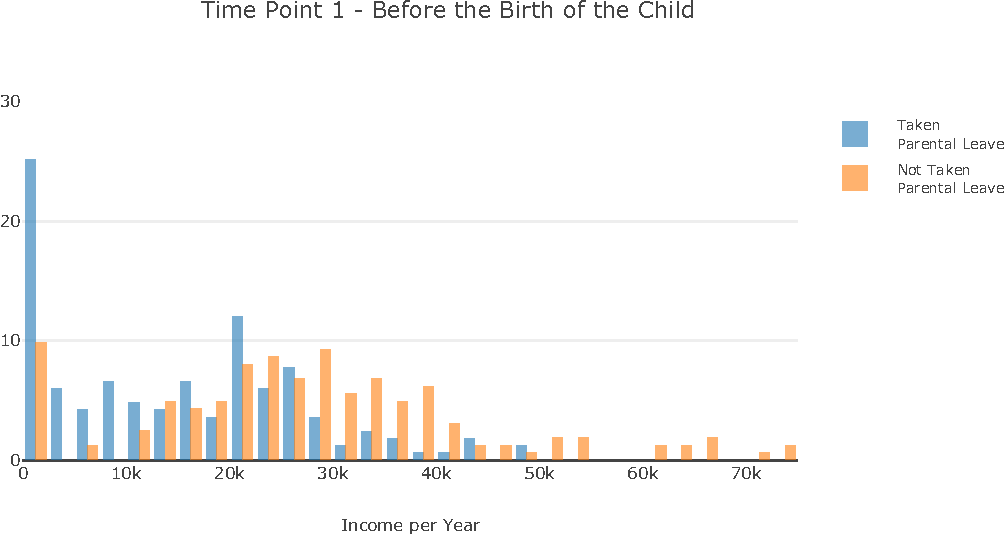
\includegraphics{Parental_Leave-Finalizing-Data-Set_files/figure-latex/fig-1-1} 

}

\caption{Distribution of Income Between Persons Taking Parental Leave or not Before the Birth of the Child (Time Point 1)}\label{fig:fig-1}
\end{figure}

\begin{figure}

{\centering 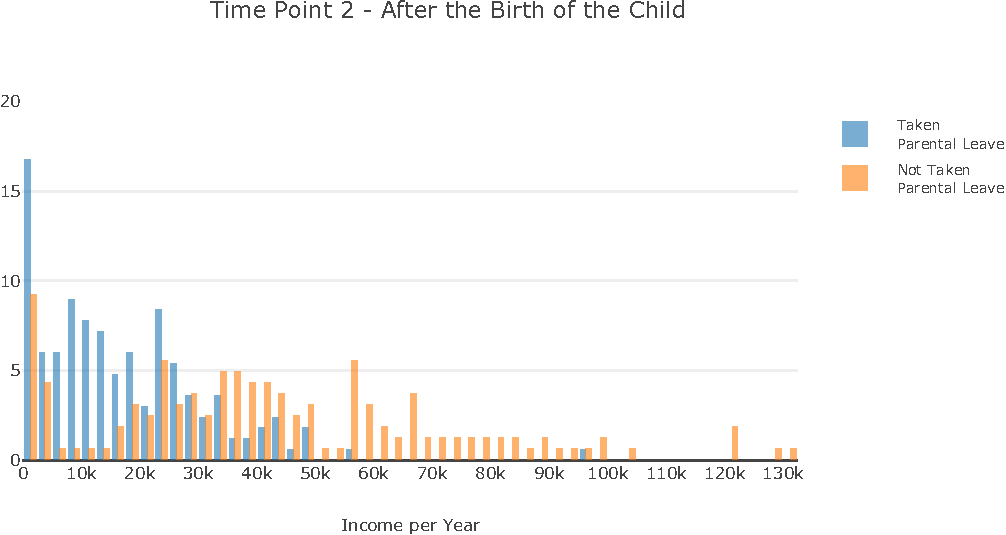
\includegraphics{Parental_Leave-Finalizing-Data-Set_files/figure-latex/fig-2-1} 

}

\caption{Distribution of Income Between Persons Taking Parental Leave or not After the Birth of the Child (Time Point 2)}\label{fig:fig-2}
\end{figure}

\hypertarget{results}{%
\section{Results}\label{results}}

\hypertarget{influence-of-parental-leave}{%
\subsubsection*{\texorpdfstring{\emph{Influence of parental leave}}{Influence of parental leave}}\label{influence-of-parental-leave}}
\addcontentsline{toc}{subsubsection}{\emph{Influence of parental leave}}

The first hypothesis I proposed was referencing to the causal influence of taking parental leave on income, especially in a long-term effect. In order to visualize the distribution of income at each time point I created a barplot shown in Figure \ref{fig:fig-1} \& \ref{fig:fig-2}. The x-axis describes the annual income for each individual and the y-axis shows the percentage.\footnote{Applies to all other graphs.} The color of the bars stand for the Individuals which took parental leave (blue) and for those who did not (orange). At time point 1, before the birth, both groups are centered around 20,000 to 30,000 euros per year. However the treatment group has more observations in the lower half and the control group is more represented in the higher income categories, indicating that there is some prior self selection, mostly due to self selection.

However, the second barplot (figure \ref{fig:fig-2}) displaying time point 2 (after birth) shows a distinct shift of both groups. The treatment group shifted towards the lower spectrum of income and the control group in the opposite direction, leaving a greater disparity between both groups. This implies that the treatment might have an impact on income.

To further examine this assumption I run a linear regression on basis of a difference in differences model shown in table \ref{tab2}. Model 1 (M1) and Model 2 (M2) display the linear regression testing the first hypothesis. M1 only tests the influence of taking parental leave on income. The results show, that if one is taking parental leave there are likely to earn 12,399.040 Euros less after 15 years compared to someone who did not take parental leave. These results are significant within a 99\% confidence interval. When introducing the control variables the results change. Taking parental leave is still significant, however the value of the coefficient decreased to -7,984.528 Euros. Comparing both models, M2 can explain 20 \% of the models variance. Therefore hypothesis 1 is not accepted within a 90\% confidence interval.

\begin{table}[!htbp] \centering 
  \caption{Regression Table - Linear Regression on Basis of a Difference in Differences Model Testing for Hypothesis 1 and 3} 
  \label{tab2} 
\footnotesize 
\begin{tabular}{@{\extracolsep{-5pt}}lcccc} 
\\[-1.8ex]\hline 
\hline \\[-1.8ex] 
 & \multicolumn{4}{c}{\textit{Dependent variable:}} \\ 
\cline{2-5} 
\\[-1.8ex] & \multicolumn{4}{c}{Annual Income} \\ 
 & M1 & M2 & M3 & M4 \\ 
\hline \\[-1.8ex] 
 Parental Leave & $-$12,399.040$^{***}$ & $-$7,984.528$^{*}$ & $-$4,889.731 & $-$3,011.547 \\ 
  & (2,099.990) & (4,661.177) & (13,537.900) & (12,904.120) \\ 
  & & & & \\ 
 Male &  & $-$7,014.564 & $-$7,832.613 & $-$6,229.043 \\ 
  &  & (4,725.737) & (4,874.618) & (5,099.879) \\ 
  & & & & \\ 
 Age &  & 3,200.347 &  & 3,186.185 \\ 
  &  & (2,057.393) &  & (2,060.677) \\ 
  & & & & \\ 
 Age Squared &  & $-$57.642$^{*}$ &  & $-$57.503$^{*}$ \\ 
  &  & (30.259) &  & (30.305) \\ 
  & & & & \\ 
 West Germany &  & $-$963.382 &  & $-$1,026.475 \\ 
  &  & (2,637.065) &  & (2,645.316) \\ 
  & & & & \\ 
 Child Count &  & 1,014.902 &  & 1,029.209 \\ 
  &  & (1,251.661) &  & (1,253.963) \\ 
  & & & & \\ 
 High Education &  & 12,396.130$^{***}$ &  & 12,468.090$^{***}$ \\ 
  &  & (2,346.398) &  & (2,356.257) \\ 
  & & & & \\ 
 Occupation &  & $-$809.866$^{**}$ &  & $-$796.397$^{**}$ \\ 
  &  & (344.886) &  & (346.922) \\ 
  & & & & \\ 
 Parental Leave X Male &  &  & $-$599.617 & $-$5,732.633 \\ 
  &  &  & (14,378.260) & (13,867.910) \\ 
  & & & & \\ 
 Constant & 14,695.790$^{***}$ & $-$25,740.850 & 15,517.730$^{***}$ & $-$25,568.090 \\ 
  & (1,496.158) & (33,832.330) & (1,579.092) & (33,884.230) \\ 
  & & & & \\ 
\hline \\[-1.8ex] 
Observations & 329 & 294 & 329 & 294 \\ 
Adjusted R$^{2}$ & 0.094 & 0.200 & 0.096 & 0.198 \\ 
\hline 
\hline \\[-1.8ex] 
\textit{Note:}  & \multicolumn{4}{r}{$^{*}$p$<$0.1; $^{**}$p$<$0.05; $^{***}$p$<$0.01} \\ 
\end{tabular} 
\end{table}

\hypertarget{length-of-parental-leave}{%
\subsubsection*{\texorpdfstring{\emph{Length of Parental Leave}}{Length of Parental Leave}}\label{length-of-parental-leave}}
\addcontentsline{toc}{subsubsection}{\emph{Length of Parental Leave}}

Figure \ref{fig:fig-3} \& \ref{fig:fig-4} show the distribution of income in relation to the length of the leave. Blue shows the treatment group (long leave) and orange the control group (short leave). As stated in hypothesis 2, I argue that the longer someone is in parental leave the higher the damage to their income. Both groups are distributed similar, they are mostly represented in the lower income field and then again around 20,000 to 30,000. This indicates that there is less pre-selection for both groups, so that the probability that both groups would develop in the same way over the 15-year period is higher.

The second graph (Figure \ref{fig:fig-4}) displays the second time point. The distribution of the treatment group generally flattened, with the majority of cases concentrated around 10,000 and 25,000. The control group, on the other hand, shows very strong variations. The percentage of those who earn up to 2500 euros per year has increased dramatically compared to time point 1, just as the percentage of those who earn around 20,000 - 25,000. There is no clear implication for whether short or long parental leaves have a stronger influence on income, however the treatment group seems to have a slightly higher income overall.
This assumption is verified by the first Model (M1) of Table \ref{tab3} which displays only the influence of the length of the parental leave on the income difference. According to the results, by taking longer parental leave (more than 6 months), the income after 15 years will be about 6,486,803 higher than for a person who has taken up to 6 months of parental leave (short leave). This result is significant within a 90 \% confidence interval. The effect stays the same after controlling. However, as the the results are not conform with the hypothesis which were proposed, hypothesis 2 has to be rejected.

\begin{figure}

{\centering 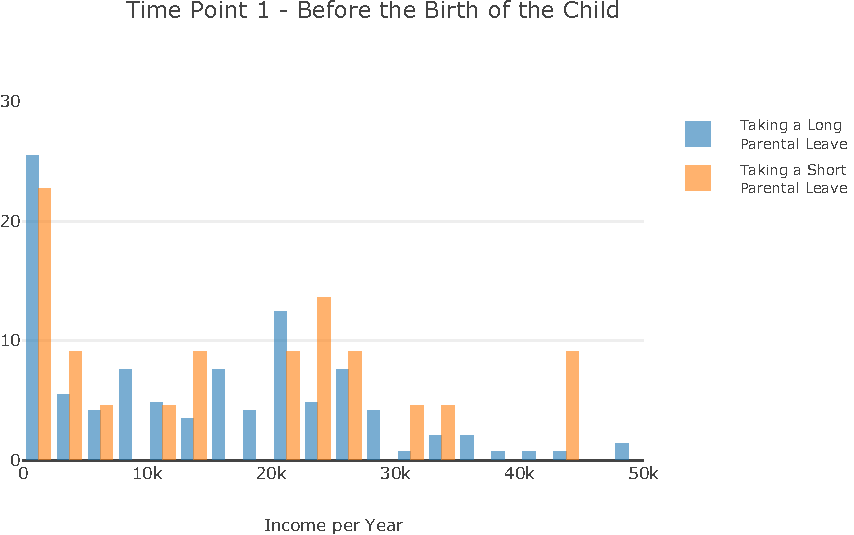
\includegraphics{Parental_Leave-Finalizing-Data-Set_files/figure-latex/fig-3-1} 

}

\caption{Distribution of Income Between Persons Taking a Long or Short Parental Leave Before the Birth of the Child (Time Point 1)}\label{fig:fig-3}
\end{figure}

\begin{figure}

{\centering 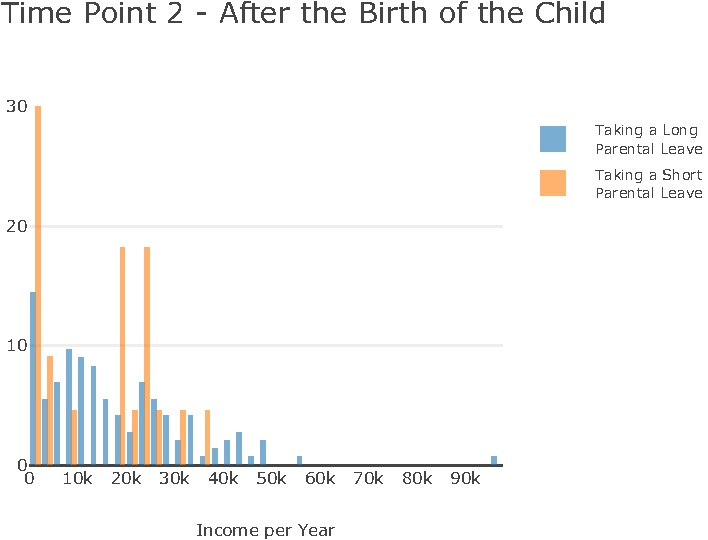
\includegraphics{Parental_Leave-Finalizing-Data-Set_files/figure-latex/fig-4-1} 

}

\caption{Distribution of Income Between Persons Taking a Long or Short Parental Leave After the Birth of the Child (Time Point 2)}\label{fig:fig-4}
\end{figure}

\begin{table}[!htbp] \centering 
  \caption{Regression Table - Linear Regression on Basis of a Difference in Differences Model Testing for Hypothesis 2} 
  \label{tab3} 
\footnotesize 
\begin{tabular}{@{\extracolsep{-5pt}}lcc} 
\\[-1.8ex]\hline 
\hline \\[-1.8ex] 
 & \multicolumn{2}{c}{\textit{Dependent variable:}} \\ 
\cline{2-3} 
\\[-1.8ex] & \multicolumn{2}{c}{Annual Income} \\ 
 & M1 & M2 \\ 
\hline \\[-1.8ex] 
 Long Leave & 6,486.803$^{*}$ & 6,016.711$^{*}$ \\ 
  & (3,624.890) & (3,341.767) \\ 
  & & \\ 
 Female &  & $-$11,455.770 \\ 
  &  & (9,967.716) \\ 
  & & \\ 
 Age &  & 9,003.787$^{***}$ \\ 
  &  & (3,030.618) \\ 
  & & \\ 
 Age Squared &  & $-$152.280$^{***}$ \\ 
  &  & (48.250) \\ 
  & & \\ 
 West Germany &  & $-$8,630.072$^{***}$ \\ 
  &  & (2,796.995) \\ 
  & & \\ 
 Child Count &  & 5,462.574$^{***}$ \\ 
  &  & (1,424.138) \\ 
  & & \\ 
 High Education &  & 4,167.398 \\ 
  &  & (2,673.758) \\ 
  & & \\ 
 Occupation &  & $-$813.028$^{**}$ \\ 
  &  & (335.953) \\ 
  & & \\ 
 Constant & $-$3,335.500 & $-$116,962.800$^{**}$ \\ 
  & (3,377.696) & (48,306.780) \\ 
  & & \\ 
\hline \\[-1.8ex] 
Observations & 167 & 153 \\ 
Adjusted R$^{2}$ & 0.013 & 0.251 \\ 
\hline 
\hline \\[-1.8ex] 
\textit{Note:}  & \multicolumn{2}{r}{$^{*}$p$<$0.1; $^{**}$p$<$0.05; $^{***}$p$<$0.01} \\ 
\end{tabular} 
\end{table}

\hypertarget{interaction-effect-between-parental-leave-and-gender}{%
\subsubsection*{\texorpdfstring{\emph{Interaction effect between Parental Leave and Gender}}{Interaction effect between Parental Leave and Gender}}\label{interaction-effect-between-parental-leave-and-gender}}
\addcontentsline{toc}{subsubsection}{\emph{Interaction effect between Parental Leave and Gender}}

Figure \ref{fig:fig-5} \& \ref{fig:fig-6} show the distribution of income by gender and participation in parental leave. Blue shows males that did parental leave, orange males that did not. Green shows the percentage of women taking parental leave and red shows the ones that continue working.
Important to note here is, that because of the general low number of observation, this is especially the case for certain subgroups in these graphs. Thus, the results might be biased.

With that said, there is a similar distribution throughout the categories for time point 1 (Figure \ref{fig:fig-5}). Most of the observations group around the 20,000 to 30,000 euros per year. Especially men who take parental leave are solely represented in these categories. Possibly because of the small observation number. In contrast, men who do not take parental leave are more wide spread and have a slightly higher income over all. This is mostly due to the fact, that men who earn a high income are less likely to go into parental leave in the first place (Döge and Volz \protect\hyperlink{ref-doge_manner_2004}{2004}). Also, there is a high number of women earning only up to 5,000 per year in this sample, especially for mothers continue to work.

Looking at the second time point (Figure \ref{fig:fig-6}), 15 years later, there are some severe changes. To start with, men which did not take parental leave had a large income increase, women who did not take parental leave on the other side did increase slightly in the higher range of income, but also increased in the lower range of income. Women who took parental leave distributed quite evenly around the 0 to 30,000 euros per year with a slight decrease towards higher income. Their male counterparts increased their income about 10,000 to 15,000 euros per year. These results imply that women compared to men will earn less in the beginning, but also when taking parental leave. However, the number of observation for men taking parental leave is really small, so the drastic difference may be caused by that.

To test the assumption that women who took parental leave had a greater decline in income, I run two regressions. First, only the interaction between gender and parental leave is displayed in Table \ref{tab2} model 3 (M3). None of the coefficients in this model are significant. The same for model 4. None of the coefficients are significant. This suggests that adding the interaction has an effect on the long term effect of parental leave. As there were no significant results found, the third hypothesis has to be rejected.

\begin{figure}

{\centering 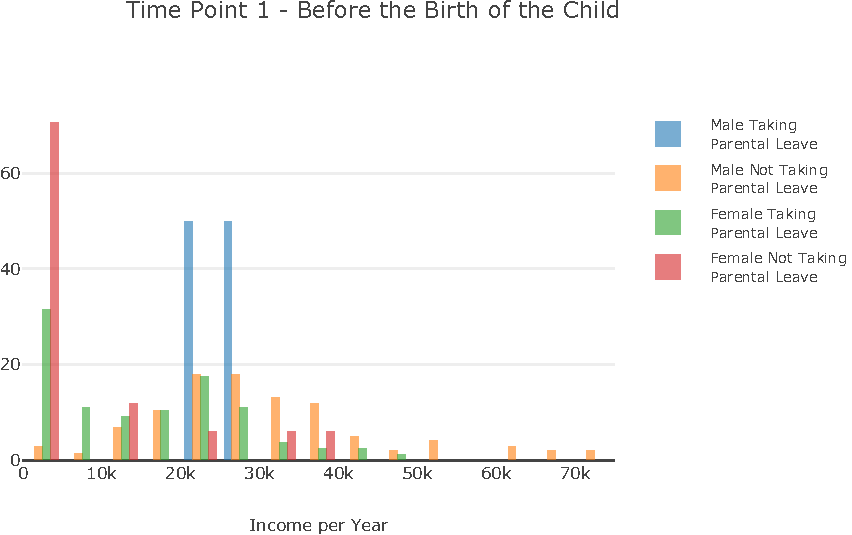
\includegraphics{Parental_Leave-Finalizing-Data-Set_files/figure-latex/fig-5-1} 

}

\caption{Distribution of Income Between Man and Women Taking Parental Leave or Not Before the Birth of the Child (Time Point 1)}\label{fig:fig-5}
\end{figure}

\begin{figure}

{\centering 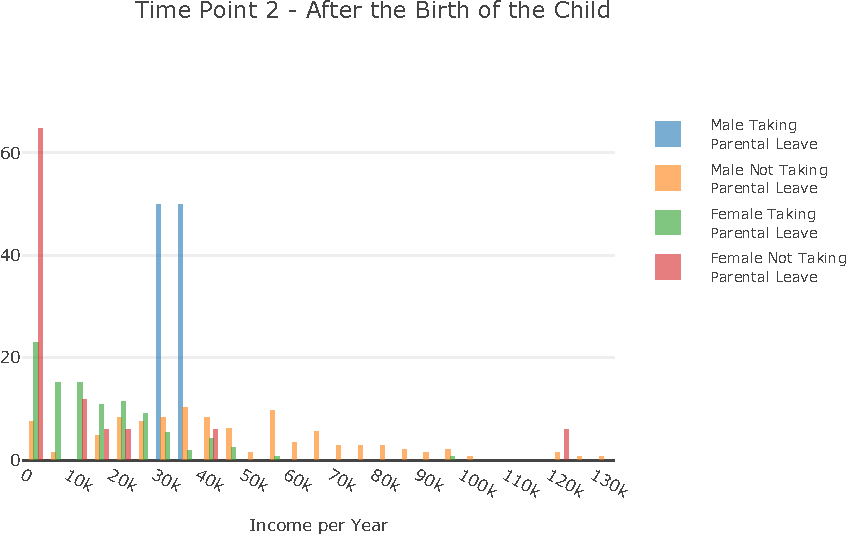
\includegraphics{Parental_Leave-Finalizing-Data-Set_files/figure-latex/fig-6-1} 

}

\caption{Distribution of Income Between Man and Women Taking Parental Leave or Not After the Birth of the Child (Time Point 2)}\label{fig:fig-6}
\end{figure}

\hypertarget{conclusion-and-discussion}{%
\section{Conclusion and Discussion}\label{conclusion-and-discussion}}

\hypertarget{conclusion}{%
\subsubsection*{\texorpdfstring{\emph{Conclusion}}{Conclusion}}\label{conclusion}}
\addcontentsline{toc}{subsubsection}{\emph{Conclusion}}

The results give contradictory implications in regards to answering the research question whether parental leave has a negative impact on future income or not. On the one hand the results regarding hypothesis 1 are in line with prior research (Evertsson \protect\hyperlink{ref-evertsson_parental_2016}{2016}; Stafford and Sundström \protect\hyperlink{ref-stafford_time_1996}{1996}). There is significant evidence that parental leave has a negative impact on future income, presumably due to missed opportunities at work and the resulting decline in human capital, leading to long lasting effects in the work field.

On the other hand, contrary to the human capital theory, I found significant results showing that a long parental leave has positive effects on the future income compared to a short leave.
I argued, that long parental leave would have a larger negative impact on the future income compared to stay for a short period of time in parental leave. However this assumption is not supported.
These results might be explained by the signalling theory. Contrary to the belief of many scholars, that parental leave would signal less commitment to the company and might imply a low work ethic in general might be true for the general impact of parental leave, additionally to the decrease in human capital (Albrecht et al. \protect\hyperlink{ref-albrecht_career_1999}{1999}; Evertsson \protect\hyperlink{ref-evertsson_parental_2016}{2016}; Stafford and Sundström \protect\hyperlink{ref-stafford_time_1996}{1996}). However, a long parental leave could be also a signal for other characteristics which might be more positive. I would argue, that if someone stays longer in parental leave, that they show determination and dedication, as they leave their job to sacrifice their career to care for their child, and this especially counts when staying for a longer period of time. Additionally, it implies openness and adaptability as carrying for a new born child is a challenging task and demand constantly adaption to new situations and be open to new possibilities to do certain tasks.
Furthermore, I did not find significant results to substantiate my third and last hypothesis. I argued that women who take parental leave have a greater disadvantage regarding their future income compared to their male counterparts. These results are most likely due to the fact, that the number of observations is really small, especially in groups like males which take parental leave. Despite the fact that they are underrepresented in this sample, it was also just not common for men to take parental leave in the mid to end 1990s.
So it is hard to make a valid statement on basis of these results.

\hypertarget{limitations-1}{%
\subsubsection*{\texorpdfstring{\emph{Limitations}}{Limitations}}\label{limitations-1}}
\addcontentsline{toc}{subsubsection}{\emph{Limitations}}

Despite of everything, there are some major shortcomings to this study. First and foremost the number of observations is really small. Which leads to a discrimination with respect to certain characteristics. Also because of this, I was not able to do a matching process which would may have helped to control for self selection. Especially in Figure \ref{fig:fig-1} (t1), we can notice a severe difference between the control and treatment group, suggesting that there was happening some sort of self selection.

Despite that, it is hard to get rid of any self selection in a natural experiment, so sometimes it is just something researcher have to deal with.
And even though I suggested in my perfect model to control the perception of couples, which might help to achieve compelte randomness, it would be highly unethical to do.

And lastly there is a large number of people who started with no income (Figure 1 - 3). Their difference which was calculated on behalf of their information might have led to a bias. For example a women who got pregnant during their studies would have had no income, however 15 years later she might have a job.
And due to the study design, her whole income is now be counted as an increase. However, I tried to counterbalance that as I only included persons which were 21 or older, so the probability that they have a job is much higher.\\
And lastly, even though I dropped all cases where someone had more than one child during the observation time period. There might been women who did more than one parental leave, however, as the variable was not featured in every wave, I could not control for that either.

\hypertarget{future-research}{%
\subsubsection*{\texorpdfstring{\emph{Future Research}}{Future Research}}\label{future-research}}
\addcontentsline{toc}{subsubsection}{\emph{Future Research}}

In regards to future research, it would be good to look at these hypothesis with a larger data set, providing more suitable observations. Additionally, it would be interesting to take an even longer period of time to really examine the long term effects. For this it might be good to use more than two time points as income fluctuates. Therefore, the course of both groups can be observed.

Another interesting point would be to look, on the one hand, at what the long-term effects would be after the 2007 reform change. But how it compares to the 1992/1993 reform.
Gabriele Mari and Cutuli (\protect\hyperlink{ref-gabriele_mari_parental_2019}{2019}) already looked at the differences between these two groups in a difference in difference model. However, they could only look at a smaller period of time.

Furthermore, the second hypothesis brings up the questions where the breaking point is regarding the length of the leave. What is the best length of parental leave in terms of the impact on income? Plantenga and Remery (\protect\hyperlink{ref-plantenga_reconciliation_2005}{2005}) belief it should be about 6-8 months. Other scholars belief that taking about longer periods than that would be better (Misra et al. \protect\hyperlink{ref-misra_work-family_2011}{2011}).

And lastly, I was wondering if there might be different results if someone adopts a child. In this case parents are allowed to take parental leave as well. The decrease in human capital would be the same, however adaption itself might send a different signal, which could be a benefit after all.
\newpage

\hypertarget{statutory-declaration}{%
\section*{Statutory Declaration}\label{statutory-declaration}}
\addcontentsline{toc}{section}{Statutory Declaration}

I hereby declare that the paper presented is my own work and that I have not called upon the help of a third party. In addition, I affirm that neither I nor anybody else has submitted this paper or parts of it to obtain credits elsewhere before. I have clearly marked and acknowledged all quotations or references that have been taken from the works of other. All secondary literature and other sources are marked and listed in the bibliography. The same applies to all charts, diagrams and illustrations as well as to all Internet sources. Moreover, I consent to my paper being electronically stores and sent anonymously in order to be checked for plagiarism. I am aware that the paper cannot be evaluated and may be graded ``failed'' (``nicht ausreichend'') if the declaration is not made.

Place, Date: Mannheim, 15.07.2020

Signature:
(Sophie Hensgen)

\newpage

\hypertarget{bibliography}{%
\section*{Bibliography}\label{bibliography}}
\addcontentsline{toc}{section}{Bibliography}

\hypertarget{refs}{}
\leavevmode\hypertarget{ref-ajdacic-gross_elterngeld_2020}{}%
Ajdacic-Gross. 2020. ``Elterngeld \& elterngeldPlus.''

\leavevmode\hypertarget{ref-albrecht_career_1999}{}%
Albrecht, James W., Per-Anders Edin, Marianne Sundstrom, and Susan B. Vroman. 1999. ``Career Interruptions and Subsequent Earnings: A Reexamination Using Swedish Data.'' \emph{The Journal of Human Resources} 34(2):294.

\leavevmode\hypertarget{ref-becker_human_1993}{}%
Becker, Gary S. 1993. \emph{Human Capital: A Theoretical and Empirical Analysis, with Special Reference to Education}. 3rd ed. Chicago: The University of Chicago Press.

\leavevmode\hypertarget{ref-desai_womens_1991}{}%
Desai, Sonalde and Linda J. Waite. 1991. ``Women's Employment During Pregnancy and After the First Birth: Occupational Characteristics and Work Commitment.'' \emph{American Sociological Review} 56(4):551.

\leavevmode\hypertarget{ref-doge_manner_2004}{}%
Döge, P. and R. Volz. 2004. ``Männer -- Weder Paschas Noch Nestflüchter: Aspekte Der Zeitverwendung von Männern Nach Den Daten Der Zeitbudgetstudie 2001/2002 Des Statistischen Bundesamtes','' \emph{Aus Politik Und Zeitgeschichte} B46:13--23.

\leavevmode\hypertarget{ref-evertsson_parental_2016}{}%
Evertsson, Marie. 2016. ``Parental Leave and Careers: Women's and Men's Wages After Parental Leave in Sweden.'' \emph{Advances in Life Course Research} 29:26--40.

\leavevmode\hypertarget{ref-gabriele_mari_parental_2019}{}%
Gabriele Mari and Giorgio Cutuli. 2019. ``Do Parental Leaves Make the Motherhood Wage Penalty Worse? Assessing Two Decades of German Reforms.'' \emph{Deutsches Institut F\textbackslash"\{u\}r Wirtschaftsforschung (DIW)} 1025:http://hdl.handle.net/10419/194106.

\leavevmode\hypertarget{ref-geisler_against_2011}{}%
Geisler, Esther and Michaela Kreyenfeld. 2011. ``Against All Odds: Fathers' Use of Parental Leave in Germany.'' \emph{Journal of European Social Policy} 21(1):88--99.

\leavevmode\hypertarget{ref-grabka_soep_2017}{}%
Grabka, Markus M. 2017. ``SOEP 2016 -- Codebook for the \$PEQUIV File 1984-2016: CNEF Variables with Extended Income Information for the SOEP.''

\leavevmode\hypertarget{ref-hakim_lifestyle_2002}{}%
Hakim, Catherine. 2002. ``Lifestyle Preferences as Determinants of Women's Differentiated Labor Market Careers.'' \emph{Work and Occupations} 29(4):428--59.

\leavevmode\hypertarget{ref-helen_dearing_does_2015}{}%
Helen Dearing. 2015. ``Does Parental Leave Influence the Gender Dividon of Labour? Recent Empirical Findings from Europe.''

\leavevmode\hypertarget{ref-hofferth_parental_2006}{}%
Hofferth, Sandra L. and Sally C. Curtin. 2006. ``Parental Leave Statutes and Maternal Return to Work After Childbirth in the United States.'' \emph{Work and Occupations} 33(1):73--105.

\leavevmode\hypertarget{ref-katherine_marshall_fathers_2008}{}%
Katherine Marshall. 2008. ``Fathers' Use of Paid Parental Leave.'' \emph{Statistics Canada} 75-001-X.

\leavevmode\hypertarget{ref-lapuerta_individual_2011}{}%
Lapuerta, Irene, Pau Baizán, and María José González. 2011. ``Individual and Institutional Constraints: An Analysis of Parental Leave Use and Duration in Spain.'' \emph{Population Research and Policy Review} 30(2):185--210.

\leavevmode\hypertarget{ref-leibowitz_employment_1992}{}%
Leibowitz, Arleen, Jacob Alex Klerman, and Linda J. Waite. 1992. ``Employment of New Mothers and Child Care Choice: Differences by Children's Age.'' \emph{The Journal of Human Resources} 27(1):112.

\leavevmode\hypertarget{ref-liebig_socio-economic_2019}{}%
Liebig, Stefan, Jan Goebel, Carsten Schröder, Markus Grabka, David Richter, Jürgen Schupp, Charlotte Bartels, Alexandra Fedorets, Andreas Franken, Jannes Jacobsen, Selin Kara, Peter Krause, Hannes Kröger, Martin Kroh, Maria Metzing, Jana Nebelin, Diana Schacht, Paul Schmelzer, Christian Schmitt, Daniel Schnitzlein, Rainer Siegers, Knut Wenzig, Stefan Zimmermann, and Deutsches Institut Für Wirtschaftsforschung (DIW Berlin). 2019. ``Socio-Economic Panel (SOEP), Data from 1984-2018Sozio-Oekonomisches Panel (SOEP), Daten Der Jahre 1984-2018.''

\leavevmode\hypertarget{ref-marshall_fathers_2008}{}%
Marshall, Katherine. 2008. ``Father's Use of Paid Parental Leave.'' \emph{Perspectives on Labour and Income} 9.

\leavevmode\hypertarget{ref-mignot_peter_2011}{}%
Mignot, J.-F. and G. Manzo. 2011. ``Peter Hedstrom and Peter Bearman (Eds.): The Oxford Handbook of Analytical Sociology.'' \emph{European Sociological Review} 27(6):824--35.

\leavevmode\hypertarget{ref-misra_work-family_2011}{}%
Misra, Joya, Michelle Budig, and Irene Boeckmann. 2011. ``Work-Family Policies and the Effects of Children on Women's Employment Hours and Wages.'' \emph{Community, Work \& Family} 14(2):139--57.

\leavevmode\hypertarget{ref-plantenga_reconciliation_2005}{}%
Plantenga, J. and Chantal. Remery. 2005. \emph{Reconciliation of Work and Private Life: A Comparative Review of Thirty European Countries.}

\leavevmode\hypertarget{ref-pronzato_return_2009}{}%
Pronzato, Chiara Daniela. 2009. ``Return to Work After Childbirth: Does Parental Leave Matter in Europe?'' \emph{Review of Economics of the Household} 7(4):341--60.

\leavevmode\hypertarget{ref-ridgeway_unpacking_2004}{}%
Ridgeway, Cecilia L. and Shelley J. Correll. 2004. ``Unpacking the Gender System: A Theoretical Perspective on Gender Beliefs and Social Relations.'' \emph{Gender \& Society} 18(4):510--31.

\leavevmode\hypertarget{ref-rostgaard_parental_2020}{}%
Rostgaard, Tine, Mogens Christoffersen, and Hanne Weise. 2020. ``Parental Leave in Denmark.''

\leavevmode\hypertarget{ref-stafford_time_1996}{}%
Stafford, Frank P. and Marianne Sundström. 1996. ``Time Out for Childcare: Signalling and Earnings Rebound Effects for Men and Women.'' \emph{Labour} 10(3):609--29.

\leavevmode\hypertarget{ref-statistisches_bundesamt_zeitreihe_2020}{}%
Statistisches Bundesamt. 2020. ``Zeitreihe: Entwicklung Des Väteranteils Nach Ländern. Destatis- Statistisches Bundesamt.''

\leavevmode\hypertarget{ref-sundstrom_gender_2002}{}%
Sundstrom, M. 2002. ``Gender Division of Childcare and the Sharing of Parental Leave Among New Parents in Sweden.'' \emph{European Sociological Review} 18(4):433--47.

\leavevmode\hypertarget{ref-tamm_fathers_2018}{}%
Tamm, Marcus. 2018. \emph{Fathers' Parental Leave-Taking, Childcare Involvement and Mothers' Labor Market Participation}. RWI.

\end{document}
